% Unofficial University of Oxford Poster Template
% https://github.com/andiac/gemini-cam
% a fork of https://github.com/anishathalye/gemini

\documentclass[final]{beamer}

% ====================
% Packages
% ====================

\usepackage[T1]{fontenc}
\usepackage{lmodern}
\usepackage[size=custom,width=36,height=48,scale=0.456]{beamerposter}
\usetheme{gemini}
\usecolortheme{ox}
\usepackage{graphicx}
\usepackage{booktabs}
\usepackage{tikz}
\usepackage{pgfplots}
\pgfplotsset{compat=1.14}
\usepackage{anyfontsize}

% ====================
% Lengths
% ====================

% If you have N columns, choose \sepwidth and \colwidth such that
% (N+1)*\sepwidth + N*\colwidth = \paperwidth
\newlength{\sepwidth}
\newlength{\colwidth}
\setlength{\sepwidth}{0.025\paperwidth}
\setlength{\colwidth}{0.3\paperwidth}

\newcommand{\separatorcolumn}{\begin{column}{\sepwidth}\end{column}}

% ====================
% Title
% ====================

\title{\Large \textbf{Robust Bayesian Inference for Postpartum Amenorrhea Duration Using Weibull Models}}

\author{\small 
    C P Yadav\inst{1}, Sachin Kumar\inst{2}, Anup Kumar\inst{2} \\
    \vspace{0.1em}
}

\institute[shortinst]{\small 
    \inst{1} Pfizer Healthcare India Pvt.Ltd., Chennai, Tamil Nadu, India \\
    \samelineand \inst{2} Department of Biostatistics and Health Informatics, SGPGIMS, Lucknow, India
}

% ====================
% Footer (optional)
% ====================

\footercontent{
\hfill
  International Workshop on Reliability Theory and Survival Analysis 2024, Organized by the Department of Statistics & DST-CIMS, Banaras Hindu University, Varanasi 
  \hfill}

% ====================
% Logo (optional)
% ====================
% Refer to https://github.com/k4rtik/uchicago-poster
% logo: https://communications.admin.ox.ac.uk/communications-resources/visual-identity/identity-guidelines/the-oxford-logo
% use this to include logos on the left and/or right side of the header:
\logoleft{
\includegraphics[height=4cm]{logo_fre.png}}
\logoright{
\includegraphics[height=3cm]{Pfizer.png}}

% ====================
% Body
% ====================
\begin{document}
\begin{frame}[t]
\begin{columns}[t]
\separatorcolumn

\begin{column}{\colwidth}
 \begin{block}{\textcolor{blue}{Introduction}}
 \textbf{Background}:
 \begin{itemize}
     \item The duration of postpartum amenorrhea (PPA) plays a critical role in reproductive health and family planning, directly impacting birth spacing decisions.
     \vspace{1mm}
     \item Recall bias in PPA studies occurs due to retrospective reporting, with durations often clustered at intervals like 3, 6, or 12 months, leading to inaccuracies. 
     \vspace{1mm}
     \item Current status data addresses this limitation by utilizing real-time information, enhancing the precision and reliability of PPA duration estimates.
 \end{itemize}
 \textbf{Objective}:
 \begin{itemize}
     \item To develop and apply robust statistical methods, informative and non-informative Bayesian estimation, for analyzing PPA duration using current status data. 
 \end{itemize}
 \end{block}

  \begin{block}{\textcolor{blue}{Methodology}}
  \textbf{Data Structure and Likelihood}:
  \begin{itemize}
    \item Each individual has a random monitoring time $C$ and event status $\delta$ where $\delta = 1$ (left-censored, $T_i \leq C_i$) if the event occurs before $C$, and $\delta = 0$ (right-censored, $T_i > C_i$) if the event occurs after $C$.    
    \vspace{1mm}
    \item The likelihood function for the parameter $\theta$ under this data setup is:
    \begin{align}\label{lik}
        L(\theta) = \prod_{i=1}^{n}[F(C_i, \theta)]^{\delta_i}[S(C_i, \theta)]^{1-\delta_i}
    \end{align}   
    \item The observed dataset for $n$ individuals is $\{(C_i, \delta_i)\}_{i=1}^n$, where $n_l = \sum_{i=1}^n \delta_i$ are left-censored and $(n - n_l)$ right-censored observations.
    \vspace{1mm}
    \item Assume $T \sim W(\alpha, \beta)$ with density and survival functions as $f(t|\alpha,\beta) = \beta \alpha t^{\alpha-1} e^{-\beta t^\alpha}$, and $S(t|\alpha,\beta) = e^{-\beta t^\alpha}$ respectively.    
\end{itemize}

\textbf{Bayesian Inference}
\begin{itemize}
    \item We assume the following independent gamma priors on the model parameters to obtain the Bayes estimator:
   \begin{align*}
	\pi_1(\alpha) = \frac{\nu_1^{\mu_1}}{\Gamma(\mu_1)} \alpha^{\mu_1 - 1} e^{-\nu_1 \alpha}; \quad \nu_1, \mu_1, \alpha > 0 \nonumber,  \\
	 \pi_2(\beta) = \frac{\nu_2^{\mu_2}}{\Gamma(\mu_2)} \beta^{\mu_2 - 1} e^{-\nu_2 \alpha}; \quad \nu_2, \mu_2, \beta > 0 
\end{align*}
\item We applied the augmentation approach that simplifies posterior inference by introducing complete likelihood based on latent variables, enabling efficient sampling with Gibbs sampling.
\vspace{1mm}
\item We introduce two latent variables for the left-censored and right-censored categories as $T_{l}^{*}$ and $T_{r}^{*}$. 
\vspace{1mm}
\item The full conditionals of $\alpha$ and $\beta$ are obtained as:
\begin{align}
     \pi_1(\alpha | \beta) &\propto \alpha^{n+\mu_1-1} \left(\prod_{i=1}^{n_l} {t^*_l}^{\alpha - 1}\right) \left(\prod_{i=n_l+1}^{n} {t^*_r}^{\alpha - 1}\right) \nonumber \\
     &\times \exp\left\{-\beta \left( \sum_{i=1}^{n_l} t^*_l + \sum_{i=n_l+1}^{n} t^*_r  + \nu_1\right)\right\}, \label{eq:alpha_conditional}\\
	\pi_2(\beta | \alpha) &\sim G\left(n + \mu_2, \sum_{i=1}^{n_l} t^*_l + \sum_{i=n_l+1}^{n} t^*_r + \nu_2\right), \label{eq:beta_conditional}	
\end{align}
\end{itemize}

\begin{itemize}
    \item Posterior samples were generated using nested Gibbs sampling, incorporating Metropolis-Hastings steps, as described by \cite{metropolis1949} and \cite{hastings1970}.
    \vspace{1.4mm}
    \item The sampling process utilized observed data along with given values of parameters and observations on latent variables to estimate the posterior distribution.
    \vspace{1.4mm}
    \item Informative and non-informative scenarios were addressed in the simulation study. 
\end{itemize}
  \end{block}
 \end{column}
\separatorcolumn

\begin{column}{\colwidth}
  \begin{block}{\textcolor{blue}{Simulation Study}}
  \begin{itemize}
      \item $T$ follows a Weibull $(\alpha = 1.35, \beta = 1.85)$ and $C$ are generated from uniform ($U[0.2, 2]$) distribution.
     \item We simulate observations for $n = 30, 50, 80$ and maintain different proportions of left- and right-censored observations at $50\%$ each.   
     \item For informative prior, we set $\mu_1=2, \nu_1=3, \mu_2=2, \nu_2=3$ and non-informative prior, we set $\mu_1=0.001, \nu_1=0.001, \mu_2=0.001, \nu_2=0.001$.  
     \item Generated $10^5$ posterior samples, with a thinning interval of 20 and an initial burn-in of 20,000 samples.
   \end{itemize}

{\small
\begin{table}[h!]
    \centering
    \caption{Parameter estimates under informative prior for different sample sizes.}
    \label{tab:results}
    \begin{tabular}{lccc}
        \toprule
            & \textbf{n=30} & \textbf{n=50} & \textbf{n=80} \\
        \midrule
        \multicolumn{4}{l}{\textbf{Point estimates}} \\
        $\alpha \ (SELF)$               & 1.26          & 1.26          & 1.26          \\
        $\beta \ (SELF)$                & 1.54          & 1.62          & 1.63          \\
        $\alpha \ (a=1)$       & 1.24          & 1.24          & 1.25          \\
        $\beta \ (a=1)$        & 1.46          & 1.56          & 1.59          \\
        $\alpha \ (a=-1)$      & 1.27          & 1.27          & 1.28          \\
        $\beta \ (a=-1)$       & 1.62          & 1.68          & 1.67          \\
        \midrule
        \multicolumn{4}{l}{\textbf{Mean Squared Error (MSE)}} \\
        $\alpha \ (SELF) $               & 0.01          & 0.01          & 0.01          \\
        $\beta \ (SELF) $                & 0.20          & 0.13          & 0.12          \\
        $\alpha \ (a=1)$       & 0.01          & 0.01          & 0.01          \\
        $\beta \ (a=1)$        & 0.24          & 0.15          & 0.13          \\
        $\alpha \ (a=-1)$      & 0.01          & 0.01          & 0.01          \\
        $\beta \ (a=-1)$       & 0.18          & 0.12          & 0.11          \\
        \midrule
        \multicolumn{4}{l}{\textbf{Bias}} \\
        $\alpha \ (SELF)$               & -0.09         & -0.09         & -0.09         \\
        $\beta \ (SELF)$                & -0.31         & -0.23         & -0.22         \\
        $\alpha \ (a=1)$       & -0.11         & -0.11         & -0.10         \\
        $\beta \ (a=1)$        & -0.39         & -0.29         & -0.26         \\
        $\alpha \ (a=-1)$      & -0.08         & -0.08         & -0.07         \\
        $\beta \ (a=-1)$       & -0.23         & -0.17         & -0.18         \\
        \midrule
        \multicolumn{4}{l}{\textbf{HPD interval}} \\
        $\alpha \ (AL)$        & 0.69          & 0.68          & 0.66          \\
        $\beta \ (AL)$         & 1.48          & 1.30          & 1.11          \\
        $\alpha \ (CP)$        & 1.00          & 1.00          & 1.00          \\
        $\beta \ (CP)$         & 0.83          & 0.89          & 0.86          \\
        \bottomrule
    \end{tabular}
\end{table}
}

{\small\begin{table}[h!]
    \centering
    \caption{Parameter estimates under non-informative prior for different sample sizes.}
    \label{tab:results2}
    \begin{tabular}{lccc}
        \toprule
             & \textbf{n=30} & \textbf{n=50} & \textbf{n=80} \\
        \midrule
        \multicolumn{4}{l}{\textbf{Point estimates}} \\
        $\alpha \ (SELF)$               & 1.30          & 1.29          & 1.30          \\
        $\beta \ (SELF)$                & 1.91          & 1.81          & 1.86          \\
        $\alpha \ (a=1)$       & 1.28          & 1.28          & 1.29          \\
        $\beta \ (a=1)$        & 1.77          & 1.73          & 1.80          \\
        $\alpha \ (a=-1)$      & 1.32          & 1.31          & 1.32          \\
        $\beta \ (a=-1)$       & 2.11          & 1.91          & 1.93          \\
        \midrule
        \multicolumn{4}{l}{\textbf{Mean Squared Error (MSE)}} \\
        $\alpha \ (SELF)$               & 0.00          & 0.01          & 0.01          \\
        $\beta \ (SELF)$                & 0.33          & 0.13          & 0.08          \\
        $\alpha \ (a=1)$       & 0.01          & 0.01          & 0.01          \\
        $\beta \ (a=1)$        & 0.26          & 0.13          & 0.08          \\
        $\alpha \ (a=-1)$      & 0.00          & 0.00          & 0.01          \\
        $\beta \ (a=-1)$       & 0.56          & 0.17          & 0.10          \\
        \midrule
        \multicolumn{4}{l}{\textbf{Bias}} \\
        $\alpha \ (SELF)$               & 0.06          & 0.07          & 0.07          \\
        $\beta \ (SELF)$                & 0.47          & 0.29          & 0.23          \\
        $\alpha \ (a=1)$       & -0.07         & -0.07         & -0.06         \\
        $\beta \ (a=1)$        & -0.08         & -0.12         & -0.05         \\
        $\alpha \ (a=-1)$      & -0.03         & -0.04         & -0.03         \\
        $\beta \ (a=-1)$       & 0.26          & 0.06          & 0.08          \\
        \midrule
        \multicolumn{4}{l}{\textbf{HPD interval}} \\
        $\alpha \ (AL)$        & 0.74          & 0.72          & 0.70          \\
        $\beta \ (AL)$         & 2.06          & 1.58          & 1.35          \\
        $\alpha \ (CP)$        & 1.00          & 1.00          & 1.00          \\
        $\beta \ (CP)$         & 0.93          & 0.97          & 0.97          \\
        \bottomrule
    \end{tabular}
\end{table}}

\begin{itemize}
  \item Informative priors reduce bias, MSE, and uncertainty, improving estimates, especially with smaller sample sizes.
  \vspace{0.5mm}
  \item Non-informative priors increase bias, MSE, and uncertainty, but their impact lessens as sample size grows.
  \vspace{0.5mm}
  \item SELF shows stable estimates with low MSE and bias, improving with sample size.
  \vspace{0.5mm}
  \item LINEX (with a=1 and a=-1) benefits from informative priors, which reduce MSE and bias compared to non-informative priors.
\end{itemize}
 \end{block} 
\end{column}
\separatorcolumn

\begin{column}{\colwidth}
  \begin{block}{\textcolor{blue}{Real Data Analysis}}
  \begin{itemize}
      \item \textcolor{magenta}{Data Source}: A subset of the NFHS-V (2020-21) dataset, specifically focusing on the duration of postpartum amenorrhea (PPA) in the district of Budaun, Uttar Pradesh, is used for the analysis \cite{nfhs5}. 
      \vspace{0.8mm}
      \item Women who had not experienced PPA at the interview were treated as right-censored, while those who had were treated as left-censored, aligning with the analysis framework. 
      \vspace{0.8mm}
      \item \textcolor{magenta}{Key Variables}: Interview date, date of last birth, and PPA indicator, with analysis restricted to women having an open birth interval (OBI) of less than 60 months for relevant and recent PPA observations.
      \vspace{0.8mm}
      \item Out of 380 women, 327 were in the left-censored category while 53 were in the right-censored category.
      \vspace{0.8mm}
      \item \textcolor{magenta}{Hyperparameters}: We calculated informative hyperparameters using the mean and sd of the data while in case of non-informative we set the same as in simulation.  
  \end{itemize}

{\small\begin{table}[h!]
    \centering
    \caption{Point and interval estimates using NFHS data.}
    \label{tab:comparison}
    \renewcommand{\arraystretch}{1.1} % Adjust row height
    \setlength{\tabcolsep}{4pt} % Adjust column spacing
    \begin{tabular}{lcc}
        \toprule
        & \textbf{Non-Informative} & \textbf{Informative} \\
        \midrule
        \multicolumn{3}{l}{\textbf{Point estimates}} \\
        $\alpha \ (SELF)$           & 0.50                  & 0.51               \\
        $\beta\ (SELF)$             & 0.56                  & 0.56               \\
        $\alpha \ (a=1)$            & 0.50                  & 0.51       \\
        $\beta\ (a=1)$              & 0.56                  & 0.56       \\
        $\alpha \ (a=-1)$           & 0.50                  & 0.51        \\
        $\beta\ (a=-1)$             & 0.56                  & 0.56        \\
        \midrule
        \multicolumn{3}{l}{\textbf{HPD}} \\
        $\alpha$      & (0.46, 0.55)        & (0.46, 0.55)     \\ 
        $\beta$       & (0.45, 0.68)        & (0.45, 0.68)     \\
        \midrule
        $mean \ duration (mo)$       & 3.28 (2.53, 4.42) &      3.28 (2.58, 4.46) \\
        \bottomrule
    \end{tabular}
\end{table}}

\begin{figure}[h!]
    \centering
    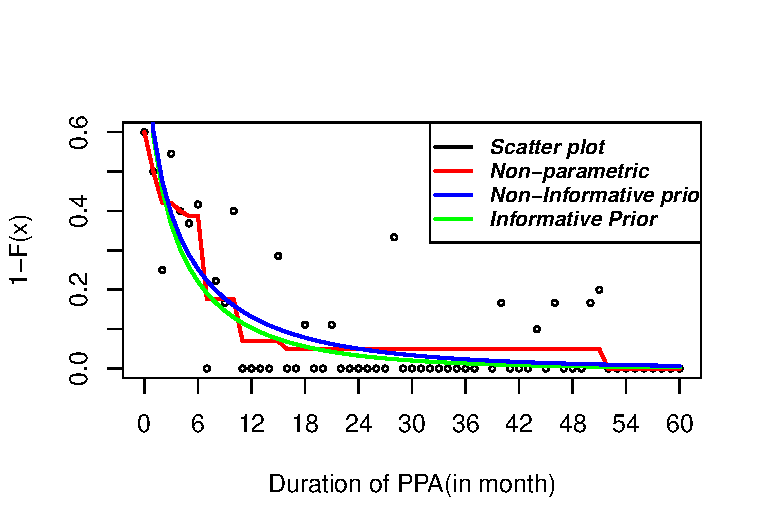
\includegraphics[width=0.9\textwidth, height=0.7\textheight, keepaspectratio]{Rplot02.pdf}
    \caption{Survival plots for the duration of PPA using different methods.}
    \label{fig:survival}
\end{figure}

 \begin{itemize}
      \item The results show consistent estimates and intervals across both priors, indicating robust parameter estimation.
      \vspace{1mm}
      \item The survival plot (Figure \ref{fig:survival}) shows smoother estimates for Bayesian methods, with slight regularization under the informative prior.
  \end{itemize}    
  \end{block}
  
  \begin{block}{\textcolor{blue}{Conclusion}}      
  \end{block}
 This study demonstrates that Bayesian estimation with current status data provides reliable and precise estimates of PPA duration, offering valuable insights for reproductive health and family planning.
  \begin{block}{\textcolor{blue}{References}}
    \nocite{*}    \footnotesize{\bibliographystyle{plain}\bibliography{poster}}
  \end{block}
\end{column}
\separatorcolumn
\end{columns}
\end{frame}
\end{document}